
%(BEGIN_QUESTION)
% Copyright 2006, Tony R. Kuphaldt, released under the Creative Commons Attribution License (v 1.0)
% This means you may do almost anything with this work of mine, so long as you give me proper credit

A level indicator is registering a liquid level that is falsely low.  The operator has hand-gauged the storage vessel with a tape measure and determined the actual level to be 9 feet, but the level indicator (LI) registers 7.5 feet.  The calibrated range of the 4-20 mA transmitter is 0 feet to 12 feet.  You measure the current signal with your multimeter and find that it is 14 mA.  Which instrument is at fault in this system?  How do you know?

$$\includegraphics[width=15.5cm]{i00321x01.eps}$$

\underbar{file i00321}
%(END_QUESTION)





%(BEGIN_ANSWER)

The transmitter is at fault, not the indicator.

%(END_ANSWER)





%(BEGIN_NOTES)


%INDEX% Basics, control loop troubleshooting
%INDEX% Calibration errors, identifying the location of in a loop
%INDEX% Measurement, level: troubleshooting

%(END_NOTES)


